\documentclass{article}
\usepackage{caption}
\usepackage{graphicx}
\usepackage{hyperref}

\title{CS 6073 Homework 4: Machine Translator}
\author{
    Luginbuhl, Dale \\
    \texttt{luginbdr@mail.uc.edu}
}
\date{November 27th 2023}


\begin{document}

\maketitle

\section{Data}
The goal of this assignment is to translate between two different
languages. More specifically, we will be translating from German to
English. We will use the \href{https://arxiv.org/abs/1605.00459}{Multi30k}
dataset for this task.

\subsection{How many data samples are included in the dataset?}
The dataset contains 31014 samples (sentences).

\subsection{Which problem will this dataset try to address?}
The dataset consists of text descriptions of images. The same images have
been described in both German and English. This allows the dataset to be
used for both multilingual image description and machine translation. We
will be focusing on the latter.

\subsection{How many words does the dataset contain?}
The training dataset contains the following:
\begin{itemize}
    \item  English: 29000 sentences, 377534 words, 13.0 words/sent
    \item  German: 29000 sentences, 360706 words, 12.4 words/sent
\end{itemize}

\subsection{Does the dataset have any missing information? E.g., missing features.}
The dataset does not have any missing information, although we are inherently limited
by the vocabulary of words that occur in the dataset.

\subsection{What is the label of this dataset?}
The dataset could be used interchangeably for machine translation from German to English,
or from English to German. We will be translating from German to English, therefore for a
given training instance, the input will be a German image description and the label
will be the corresponding English description.

\subsection{How many percent of data will you use for training, validation and testing?}
The dataset is pre-split into training, validation, and testing sets. The
training dataset contains 29000 samples (sentences), while the validation
and test datasets contain 1014 and 1000 samples respectively.

The resulting percentage splits will then be:
\begin{itemize}
    \item Training : 93.5\%
    \item Validation : 3.3\%
    \item Test : 3.2\%
\end{itemize}

\subsection{What kind of data pre-processing will you use for your training dataset?}

We treat our training samples (sentences) as a sequence of words. We will first tokenize
our sequence using a pretrained pipeline model from spaCy. We use en\_core\_web\_sm for our
English pipeline, and we use de\_core\_news\_sm for our German pipeline. Next we build a
vocabulary for each language based on the set of tokens for the language. We encode
each token in the sequence as an integer representing the index of the token in the
vocabulary. Finally, we prepend the sequence with an encoded beginning-of-sentence (BOS)
token, and append the sequence with an encoded end-of-sentence (EOS) token.


\section{Model}
We chose a Seq2seq Transformer model similar to that introduced in the
\href{https://arxiv.org/abs/1706.03762}{"Attention is all you need"} paper. To evaluate
our model we will be using a normalized BLEU score.

\section{Objective}
We will use cross-entropy loss to train the model.

\section{Optimization}
We chose the Adam optimizer to take advantage of momentum in our optimization.
Adam allows us to converge to an optimum value more quickly, and it allows
provides the potential to escape from local minima.

\section{Model Selection}
The model selected used an embedding size of 512, 8 attention heads, 3 encoder
layers, 3 decoder layers, and a hidden dimension of 512 in the feedforward
network of the transformer. We also applied dropout with a probability of 0.1
for regularization.

\section{Model Performance}

\begin{table}[h]
\begin{center}
\begin{tabular}{c|c|c}
    Model & BLEU \\
    \hline
    Seq2seq Transformer & 0.28174 \\
\end{tabular}
\end{center}
\caption{Model Evaluation}
\label{table:evaluation_matrix}
\end{table}

\begin{figure}[h]
    \centering
    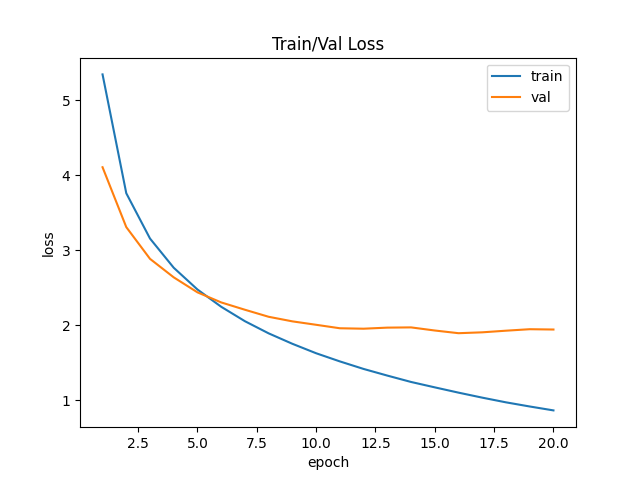
\includegraphics[width=1.0\textwidth]{./images/train_val_loss.png}
    \caption{Seq2seq Transformer training and validation loss}
    \label{fig:loss_plot}
\end{figure}

\begin{figure}[h]
    \centering
    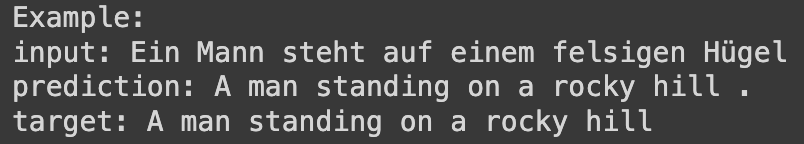
\includegraphics[width=1.0\textwidth]{./images/translation_example.png}
    \caption{Example translation}
    \label{fig:translation_example}
\end{figure}

Our model acheived modest performance with a BLEU score of 0.28174 or
28.174\% as seen in Table \ref{table:evaluation_matrix}. Using the following
\href{https://cloud.google.com/translate/automl/docs/evaluate#interpretation}{interpretation provided by Google},
a BLEU score in the range of 20-29 signifies that ``The gist is clear, but has
significant grammatical errors''. This interpretation was reinforced as we
tried example translations. One instance can be seen in Figure \ref{fig:translation_example},
where the translator added a superfluous ``.'' with incorrect spacing.

It can be seen in Figure \ref{fig:loss_plot} that the model began to overfit
around 18 epochs. To mitigate this we could experiment with more aggressive
dropout probabilities, but even better would be to increase the amount of
training data. This would likely allow us to achieve a higher BLEU score, as
well as allow the translator to work in a larger number of contexts.

\end{document}
